\documentclass[11pt]{article}
\usepackage{amssymb, amsmath, libertine, hyperref, xcolor, booktabs, enumitem, microtype}
\usepackage[T1]{fontenc}
\usepackage[margin=1in]{geometry}
\usepackage{tikz}
\newcommand{\gridxy}[4]{%
  \foreach \gX in {#1,...,#2} \draw[gray!25] (\gX,#3) -- (\gX,#4);
  \foreach \gY in {#3,...,#4} \draw[gray!25] (#1,\gY) -- (#2,\gY);}
\definecolor{dark-red}{rgb}{0.4,0.15,0.15}
\definecolor{blue-g}{rgb}{0.15,0.28,0.45}
\hypersetup{colorlinks, linkcolor=dark-red, urlcolor=dark-red}
\setlist[enumerate,1]{label=\textbf{(\alph*)}, leftmargin=*, itemsep=7pt, topsep=5pt}
\pagestyle{empty}
\newcommand{\prob}[1]{\bigskip\noindent\textbf{\large #1}\par\smallskip}

\begin{document}
\begin{center}
{\Large\bfseries Math 111: Calculus \quad Practice Exam 1 --- Solutions}
\end{center}

\medskip
\noindent These are written out in full. On the exam you would not need this much prose ---
but you would need the \emph{reasons}, and every reason here is one that earns marks.

\bigskip\hrule

%%%%%%%%%%%%%%%%%%%%%%%%%%%%%%%%%%%%%%%%%%%%%%%%%%%%%%%%%%%%%%%%%%%%%%%%%%%%%%%%
\prob{1. The definition, by hand}

\begin{enumerate}
\item With $f(x)=x^2-3x$ we have $f(2) = 4-6 = -2$, and
\[
f(2+h) = (2+h)^2 - 3(2+h) = 4 + 4h + h^2 - 6 - 3h = h^2 + h - 2 .
\]
So
\[
\frac{f(2+h)-f(2)}{h} \;=\; \frac{(h^2+h-2) - (-2)}{h} \;=\; \frac{h^2+h}{h} \;=\; h+1 ,
\]
where the cancellation is legitimate because $h \neq 0$ at every stage --- we are looking at
what happens \emph{as} $h$ approaches $0$, never at $h=0$ itself. Therefore
\[
f'(2) = \lim_{h\to 0}(h+1) = \boxed{1}.
\]

\item For an arbitrary $a$,
\[
f(a+h)-f(a) = \big[(a+h)^2 - 3(a+h)\big] - \big[a^2-3a\big] = 2ah + h^2 - 3h ,
\]
so the difference quotient is $2a + h - 3$ and
\[
f'(a) = \lim_{h\to 0}(2a+h-3) = 2a-3 .
\]
Setting $a=2$ gives $f'(2) = 4-3 = 1$, which agrees with part (a).

\item $f'(2)=1$ says the tangent line to the graph at the point $(2,-2)$ has slope $1$: at
that instant $f$ is increasing, and it is rising by about one unit of output for each unit
of input.
\end{enumerate}

%%%%%%%%%%%%%%%%%%%%%%%%%%%%%%%%%%%%%%%%%%%%%%%%%%%%%%%%%%%%%%%%%%%%%%%%%%%%%%%%
\newpage
\prob{2. Everything from one picture}

\begin{enumerate}
\item Reading slopes off the picture: on $(0,2)$ the graph rises but flattens as it goes, so
$f'$ is positive and decreasing, from roughly $1.8$ down to roughly $0.7$. On $(2,4)$ the
graph is a straight line falling two units over two, so $f' = -1$ exactly. After $x=4$ the
fall eases, $f'$ passes through $0$ at the low point $x=5$, and then the graph climbs ever
more steeply, so $f'$ rises to about $2$ by $x=7$. At $x=2$ there is no value of $f'$ at all.

\smallskip
\begin{center}
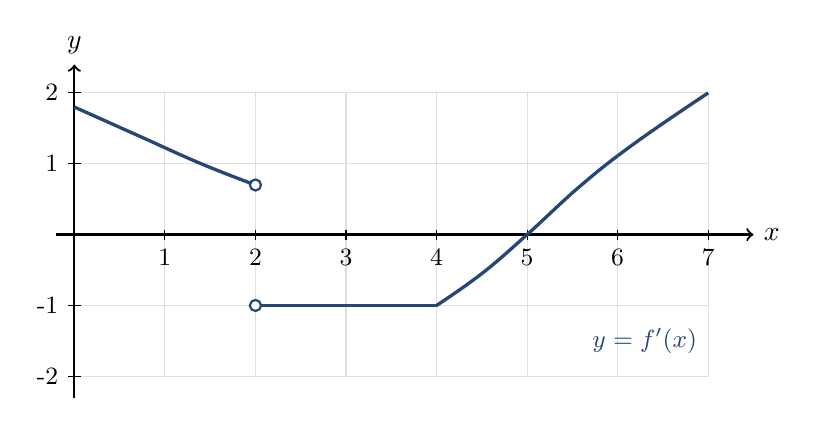
\begin{tikzpicture}[x=1.15cm,y=0.9cm]
  \gridxy{0}{7}{-2}{2}
  \draw[->,thick] (-0.2,0) -- (7.5,0) node[right] {$x$};
  \draw[->,thick] (0,-2.3) -- (0,2.4) node[above] {$y$};
  \foreach \x in {1,...,7} \draw (\x,0.07) -- (\x,-0.07) node[below,font=\small] {\x};
  \foreach \y in {-2,-1,1,2} \draw (0.07,\y) -- (-0.07,\y) node[left,font=\small] {\y};
  \draw[very thick, blue-g, smooth, tension=0.7]
    plot coordinates {(0,1.8) (0.7,1.4) (1.4,1.0) (2,0.7)};
  \draw[very thick, blue-g] (2,-1) -- (4,-1);
  \draw[very thick, blue-g, smooth, tension=0.7]
    plot coordinates {(4,-1) (4.5,-0.55) (5,0) (5.6,0.7) (6.2,1.3) (7,2.0)};
  \fill[white,draw=blue-g,thick] (2,0.7) circle (2pt);
  \fill[white,draw=blue-g,thick] (2,-1) circle (2pt);
  \node[blue-g,font=\small] at (6.3,-1.5) {$y=f'(x)$};
\end{tikzpicture}
\end{center}
The open circles at $x=2$ record that $f'(2)$ does not exist: the values approach $0.7$ from
the left and $-1$ from the right, and neither is ``the'' derivative.

\item \textbf{$f'$ fails to exist at $x=2$, and only there.} Approaching from the left the
difference quotients approach about $0.7$; approaching from the right they approach $-1$.
Since the one-sided limits disagree, the two-sided limit defining $f'(2)$ does not exist ---
there is no single tangent line at that point, because the graph has a corner.

\textbf{But $f$ \emph{is} continuous at $x=2$.} The graph has no break or jump there: both
pieces meet at the height $f(2)=3$, so $\lim_{x\to2}f(x) = 3 = f(2)$. This is the
$g(x)=|x|$ situation: continuity does not buy you differentiability. The implication runs
one way only.

\item \textbf{$f'$ is increasing on $(4,7)$.} Justifying this from the graph of $f$ itself:
on $(0,2)$ the curve rises but bends \emph{downward} --- each unit of $x$ buys less height
than the one before --- so its slope is falling and $f'$ is decreasing there. On $(2,4)$ the
graph is a straight line, so its slope is the same everywhere: $f'$ is \emph{constant} on
that stretch, neither increasing nor decreasing. On $(4,7)$ the curve bends upward: it falls
less and less steeply, levels off, and then climbs more and more steeply, so its slope is
growing the whole way.

\item \textbf{$f'(3) < f'(5) < f'(1)$.}

No numbers are needed. At $x=3$ the graph is falling, so $f'(3)<0$. At $x=5$ the graph is at
its lowest point and momentarily flat, so $f'(5)=0$. At $x=1$ the graph is rising, so
$f'(1)>0$. A negative number, then zero, then a positive number.

(For the record, $f'(3)=-1$ exactly, since that part of the graph is a straight line, and
$f'(1)$ is around $1.2$.)
\end{enumerate}

%%%%%%%%%%%%%%%%%%%%%%%%%%%%%%%%%%%%%%%%%%%%%%%%%%%%%%%%%%%%%%%%%%%%%%%%%%%%%%%%
\newpage
\prob{3. A reservoir, and what the numbers are worth}

It pays to compute the average rates of change first, in millions of gallons per day:

\smallskip
\begin{center}
\begin{tabular}{@{}lrrrr@{}}
\toprule
interval & $[0,3]$ & $[3,6]$ & $[6,9]$ & $[9,12]$\\
average rate & $0.30$ & $0.20$ & $0.10$ & $0.03$\\
\bottomrule
\end{tabular}
\end{center}

\begin{enumerate}
\item Use the central difference, which uses data on both sides of $t=6$:
\[
V'(6) \;\approx\; \frac{V(9)-V(3)}{9-3} \;=\; \frac{5.8-4.9}{6} \;=\; 0.15
\quad\text{millions of gallons per day.}
\]
The units come from the difference quotient itself: millions of gallons on top, days on the
bottom. In words: \emph{six days into September the reservoir is gaining water at about
$150{,}000$ gallons a day.}

\item The average rate over $[3,6]$ is $0.20$ and over $[6,9]$ is $0.10$.

The table shows the reservoir filling more and more slowly, so $V'$ is \textbf{decreasing}.
Every instantaneous rate on $[3,6]$ is therefore at least as large as $V'(6)$, and the
average of those rates --- the secant slope $0.20$ --- is at least $V'(6)$ too. So
$\mathbf{0.20}$ \textbf{is the over-estimate}. By the same reasoning every rate on $[6,9]$
is at most $V'(6)$, so $\mathbf{0.10}$ \textbf{is the under-estimate}:
\[
0.10 \;\le\; V'(6) \;\le\; 0.20 .
\]
The assumption doing the work is that $V'$ is decreasing throughout $[3,9]$ --- that the
filling slows steadily and never speeds back up. The table supports it, but the table only
shows every third day, so this is an assumption about what happens in between rather than
something the data proves.

Notice that the estimate from part (a) sits exactly at the midpoint of this interval, so it
is off by at most $0.05$ million gallons per day.

\item $V'$ is \textbf{decreasing}: the average rates run $0.30, 0.20, 0.10, 0.03$, all
positive but shrinking.

So the reservoir is still filling, but it is filling more and more slowly --- it is
levelling off. Whoever manages it should not plan on much more water arriving from this
source; over the last three days it gained only about $100{,}000$ gallons in total, against
$900{,}000$ in the first three.
\end{enumerate}

%%%%%%%%%%%%%%%%%%%%%%%%%%%%%%%%%%%%%%%%%%%%%%%%%%%%%%%%%%%%%%%%%%%%%%%%%%%%%%%%
\prob{4. The tangent line as an approximation}

\begin{enumerate}
\item The tangent line at $x=4$ passes through $(4,12)$ with slope $-0.8$:
\[
L(x) = 12 - 0.8(x-4).
\]
Hence $f(4.5) \approx L(4.5) = 12 - 0.8(0.5) = \boxed{11.6}$.

\item \textbf{It is too large.} Because $f$ is concave down near $x=4$, its graph bends away
below the tangent line on both sides of the point of tangency, so the line sits above the
curve and $L(4.5) > f(4.5)$.

\smallskip
\begin{center}
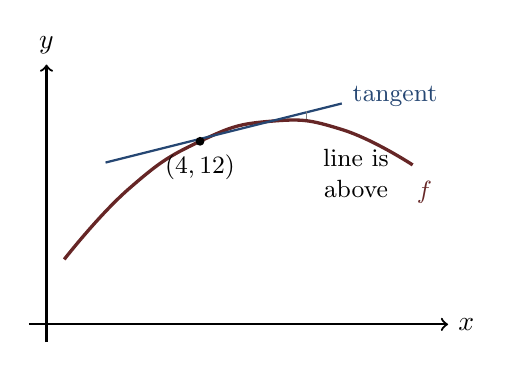
\begin{tikzpicture}[x=1.5cm,y=1.5cm]
  \draw[->,thick] (-0.15,0) -- (3.4,0) node[right] {$x$};
  \draw[->,thick] (0,-0.15) -- (0,2.2) node[above] {$y$};
  \draw[very thick, dark-red, smooth, tension=0.8]
    plot coordinates {(0.15,0.55) (0.7,1.15) (1.3,1.55) (1.9,1.72) (2.5,1.65) (3.1,1.35)};
  \draw[thick, blue-g] (0.5,1.37) -- (2.5,1.87);
  \fill (1.3,1.55) circle (1.6pt);
  \draw[dashed,gray] (2.2,1.805) -- (2.2,1.70);
  \node[font=\small] at (1.3,1.33) {$(4,12)$};
  \node[blue-g,font=\small] at (2.95,1.93) {tangent};
  \node[dark-red,font=\small] at (3.2,1.12) {$f$};
  \node[font=\small,align=center] at (2.62,1.28) {line is\\above};
\end{tikzpicture}
\end{center}

\item The method does not break down --- you can certainly write $L(9) = 12-0.8(5) = 8$ ---
but you should not trust the number. A tangent line matches $f$ well only \emph{near} the
point of tangency, and with $f$ concave down the curve peels further below the line the
further you go. At $x=4.5$ you have travelled half a unit; at $x=9$ you have travelled five,
ten times as far, and the accumulated error can be enormous. Worse, you were told about the
concavity only \emph{near} $x=4$, so you know nothing at all about the shape of $f$ out at
$x=9$ --- it may have turned around several times.

To trust such an estimate you would need to know that $f$ continues to behave over the whole
interval $[4,9]$ --- specifically, some bound on how fast $f'$ is allowed to change across
it. Failing that, the honest move is to get a data point closer to $9$.
\end{enumerate}

\end{document}
